\par Silicon Photonics supports weighted summation through constructive and destructive interference of waveguide confined light, can be assembled into a grid/mesh structure with nodes that route light, and light sources and light detectors that are able to set boundary conditions and readout solutions. Due to these similarities it is tempting to assume an equivalence exists between the Electrical Mesh introduced in Section \ref{electricalPDE}, however we will show that there are fundamental physical differences between how the Photonic node behaves compared to the electrical node. Despite these differences Silicon Photonics has established fabrication procedures both internally at the \acrfull{open} Lab and GW \acrfull{nic} as well as externally at commercial foundries including the \acrfull{aim photonics}. The physics of Metatronic ROC discussed in Section \ref{metatronicPDE} encompass a better mapping to the Electrical Difference equation in Section \ref{electricalPDE} but current Metatronic fabrication processes are in there infancy and are currently done at length scales \cite{estakhri2019inverse} orders of magnitude greater than what is needed for our Nanoscale Metatronic ROC implementation. The combination of imperfect mapping and feasible fabrication make Photonic ROC worthy of understanding and implementing as a way to showcase current capabilities of optical analog computing. 

%\subsection{Physics of Operation}

\subsection{Limitations of Passive Photonic Difference Equation Approximation}

\par Photonic ROC operates in the optical band at $\lambda = \SI{1550}{n\meter}$ with waveguide and optical splitter dimensions in length scale order of micrometers, far larger than the operating wavelength of light, resulting in \gls{distributed element model} characteristics for the optical circuit. Current fabricated Photonic \acrshort{roc} is passive with a future active Photonic ROC planned to be fabricated at \acrshort{aim photonics}.

\par Initial experimental fabrications of Photonic ROC have been composed of pure silicon and have been \gls{passive optical} circuits, meaning that waveguide geometry is the driving force for circuit behaviour. 


\par Although there is no photonic equivalent of electrical inductance or capacitance at micrometer length scales, optical loss due to waveguide attenuation can be considered analogous to electrical current resistance. The fixed optical loss fabricated into waveguide geometries allows for passive photonic ROC to approximately solve Laplace class \acrshort{pde}s.

\par Unlike the electrical mesh, each Photonic ROC splitting node, composed of 4 ring resonators and a central splitter, due to its micrometer size and distributed element model behavior is effectively isolated from its neighborhood of surrounding nodes due to the limit of what a single wavelength of light can reach in a discrete time step. 

\par Computationally this means that at a single point in time the only physical effect that determines how much light is sent into each of three possible waveguides or is reflected back into the originating waveguide is the geometry of the node which is fixed. Irregardless of boundary conditions set and inbound light from surrounding waveguides, each optical node will always split light in the same percentages, determined by its geometry. This physics is fundamentally different from the splitting occurring in the electrical mesh in Section \ref{electricalPDE} and Metatronic ROC in Section \ref{metatronicPDE} in which each node's "visibility", due to their lumped circuit behavior, operates as an all to all network at any given time step. In a finite difference algorithm that relies on a nodes immediate neighborhood to calculate the measured value at a node, the neighborhood visibility of a single node is paramount. The effects of the photonic splitting paradigm will be explored but first it is important to understand the path that light travels through a node.

\par As light enters the node a percentage is coupled into the left and right ring resonators on either side of the waveguide prior to entering the central square where the light  is reflected off of the central circular cavity with an eventual archived splitting of roughly $33\%$ of the light traveling into each of the three surrounding waveguides as shown in Figure \ref{fig:photonic_metatronic_simulations}. The design process, physics, and geometry of this novel splitter will be covered in depth in the dissertation and future Photonic ROC fabrication paper of PhD candidate and OPEN Lab member Shuai Sun.

\begin{figure}[ht]
\centering\fbox{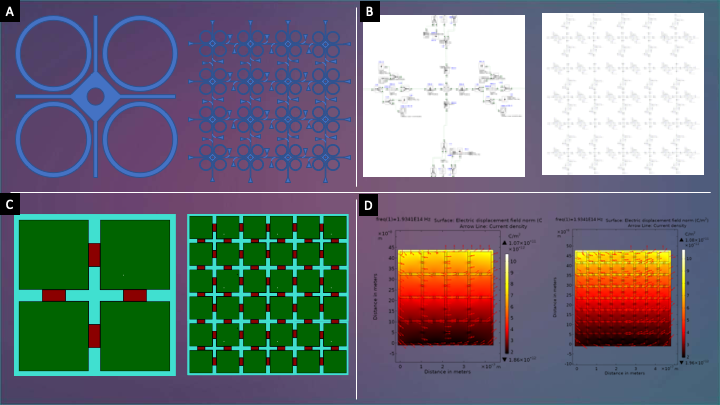
\includegraphics[height=3in, width=5.5in]{figures/figures2/04_phot_mt_models.png}}
\caption{The \textbf{(A)} geometrically engineered fixed optical loss fabricated into waveguide geometries allows for \textbf{(B)} Lumerical INTERCONNECT passive photonic \acrshort{roc} simulations to approximately solve Laplace class \acrshort{pde}s. However, unlike the electrical mesh, each photonic \acrshort{roc} splitting node, composed of 4 ring resonators and a central splitter, due to its micrometer size and distributed element model behavior is effectively isolated from its neighborhood of surrounding nodes due to the limit of what a single wavelength of light can reach in a discrete time step. The \textbf{(C)} metatronic splitting is neighborhood defined and can be \textbf{(D)} simulated with COMSOL to showcase the \acrshort{enz} confinement of displacement current density.}
\label{fig:photonic_metatronic_simulations}
\end{figure}

\par The difference equation mapping for Photonic ROC is the same as the electrical mesh up to Equation \ref{eq:3}. Once Physics becomes involved in the mapping, the first step is for current summation from the electric mesh described in Equation \ref{eq:6} to roughly map the optical intensity measured by the sum of the output grating couplers attached to each output waveguides of each splitters written as 
 
\begin{dmath}\label{eq_lightDual}
	\sum_{n=1}^{4} P_n = 0 
\end{dmath}

where $P_n$ is the optical intensity measured at each of the output grating couplers of each node.